\section{Этикет и правила поведения}

В данном разделе описываются общепринятые правила поведения и этикета, которые позволяют играть более быстро и ясно, делать меньше ошибок и провоцировать меньше спорных ситуаций. Мы рекомендуем придерживаться этих правил в любой игре --- ваши оппоненты будут вам благодарны. Некоторые пункты следует принять как обязательные --- в некоторых случаях нарушение рекомендаций может повлечь за собой вежливое указание от судьи или даже штраф. О потенциальных последствиях несоблюдения рекомендаций будет написано отдельно в каждом пункте, кроме того можно также заглянуть в раздел о судейских регламентах для уточнений.

Основные рекомендации в процессе игры --- это с одной стороны не спешить и успевать делать все четко, с другой --- не затягивать раздачу. 

\subsection {Начало игры}

Некоторые игроки при постройке стены ставят дальний ряд на ближний и делают это у борта. Некоторые техники жульничества основаны на том, что проще закладывать себе тайлы для подмены на верхний ряд, поэтому лучше будет отодвинуть оба ряда от борта и поставить ближний ряд сверху верхнего. Однако и это не лучший способ --- в процессе отодвигания стена может порушиться и придется перемешивать тайлы и набирать заново. Поэтому наиболее быстрый и надежный способ построения стены следующий: набираем два ряда по 17 у борта, равняем их, аккуратно отодвигаем дальний ряд туда, где будет стоять стена, отодвигаем ближний ряд от борта, после чего (желательно по частям) ставим поверх дальнего ряда. 

Отодвигать ряд стены следует движениями влево-вправо, чтобы исключить возможность разрушения построенного ряда.

После построения стены желательно слегка повернуть ее так чтобы правый ряд был чуть выдвинут вперед:

\begin{figure}[H]
	\centering
	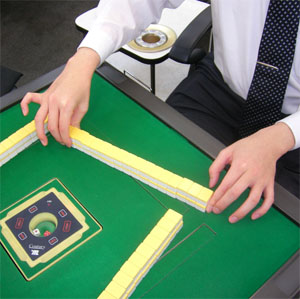
\includegraphics[width=8cm]{etiquette-1.png}
	\caption{Расположение стены}
\end{figure}

Это нужно, во-первых, чтобы тоймену было чуть проще тянуться за тайлом (чтобы по мере разбора ему тянуться не стало сложнее рекомендуется пододвигать свою стену время от времени), во-вторых, чтобы игроку слева было видно, есть ли в нижнем ряду тайл --- когда стена параллельно его взгляду увидеть тайл сложно. Двигать стену рекомендуется до броска кубиков, т.к. формально, бросок кубиков это начало раздачи, и случайное разрушение стены после него может наказываться штрафом чомбо. 

Перемешивание тайлов, построение стены и сортировка тайлов в своей руке (как при наборе тайлов так и во время игры) --- это действия, которые можно и нужно делать двумя руками, однако дальнейшие действия следует выполнять одной рукой (желательно доминантной).

В некоторых источниках рекомендуют также делать разлом стены «лесенкой» 6-5-6, однако в других источниках напротив рекомендуют от этой практики отказаться:

\begin{figure}[H]
	\centering
	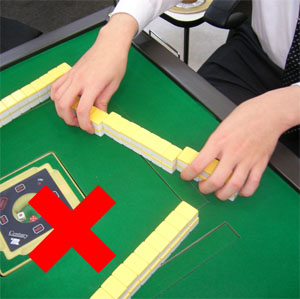
\includegraphics[width=8cm]{etiquette-2.png}
	\caption{Стена лесенкой}
\end{figure}

Считается, что такой разлом позволяет дилеру проще понять где нужно сделать разлом, но это может не сработать, если самому сделать сдвиги неправильно. Другие аргументы за сдвиг:
\begin{itemize}
	\item В сдвинутой стене если случайно толкнуть верхний ряд --- не упадет верхний тайл на другом конце стены.
	\item Сдвиг делают чтобы показать что не собираются жульничать (манипуляции с такой стеной крайне затруднительны и намного более очевидны).
\end{itemize} 
В итоге однозначных доводов против разлома нет, однако требовать этого от всех игроков затруднительно, так что решение о сдвиге остается за игроком.

\subsubsection{Бросок кубиков, разлом, мертвая стена}

После броска кубиков дилером рекомендуется вслух проговорить выброшенное число, убедиться, что все игроки увидели то же самое (бывают случаи когда кому-то показалось другое число), и сразу же забрать и отложить кубики в правый угол стола. Обратите внимание, что именно кубики обозначают текущего дилера в раздаче, а не индикатор раунда. Индикатор раунда является также индикатором первого дилера, он должен лежать у игрока который являлся первым дилером в ханчане (тонпусене) и не перемещаться во время игры (только переворачиваться в начале южного раунда). 

Разлом стены может выполнить игрок на чью стену указал бросок кубиков, также разлом может выполнить дилер одновременно со своим первым взятием. Обратите внимание что тк стена всегда содержит 17 тайлов, то, когда на кубиках выброшено больше 8 --- проще отсчитать остаток с левой части стены --- например 7, когда выброшено 10, или 5, когда выброшено 12. 

Игрок в чьей стене находится изначальный индикатор доры должен перевернуть ее, не замедляя процесса набора тайлов (если до него дошла очередь взять тайлы, то следует сначала взять их, а потом пока берут другие игроки, открыть индикатор). Остальные действия являются опциональными: снятие первого тайла замены в мертвой стене --- действие не обязательное, но рекомендуемое:

\begin{figure}[H]
	\centering
	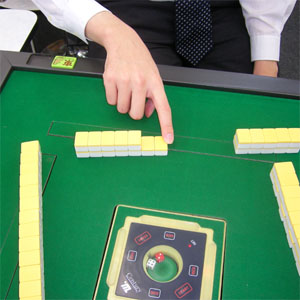
\includegraphics[width=8cm]{etiquette-3.png}
	\caption{Мертвая стена}
\end{figure}

Снятый тайл замены может остановить случайное взятие тайла не с того конца стены, т.к. мертвая стена будет визуально отличаться от живой, намекая что брать из нее не следует. При желании также можно отделить мертвую стену от живой, сделав небольшой разлом, опять же не замедляя процесс набора тайлов.

Впрочем следует помнить что большая часть раздач не доходит до ничьей, поэтому беспокоится о том когда закончится живая стена раньше середины третьей полоски нет смысла, кроме того, за раздачу могут быть объявлены каны, поэтому изначальный разлом может стать неактуальным. В общем, не рекомендуется тратить на это время раньше, чем это необходимо.

Наконец, недопустимо передвигать тайлы из одной стены в другую с целью полностью отделить мертвую стену --- это бессмысленная трата времени, которая еще и иногда приводит к тому, что у игрока в стене оказывается слишком много тайлов (и такую стену банально неудобно двигать). Общий совет тут --- избегайте трогать тайлы в чужой стене кроме случаев взятия в свой ход. За попытку передвигать тайлы из чужой стены в свою и наоборот может последовать вежливое указание так не делать.

\begin{figure}[H]
	\centering
	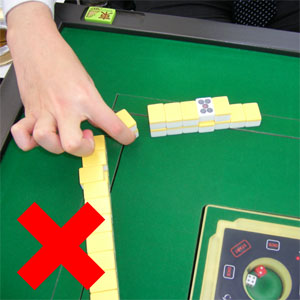
\includegraphics[width=8cm]{etiquette-4.png}
	\caption{Не трогайте чужие стены}
\end{figure}

\subsubsection{Набор тайлов}

Не рекомендуется набирать все тайлы рубашкой вверх и затем открывать всю руку:

\begin{figure}[H]
	\centering
	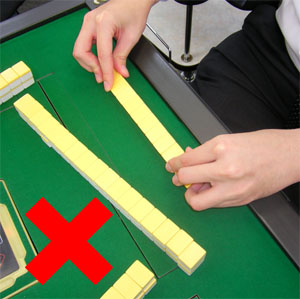
\includegraphics[width=8cm]{etiquette-5.png}
	\caption{Набор тайлов со стены}
\end{figure}

Это может привести к тому что некоторые тайлы будут вскрыты (в лучшем случае), а ближайшая стена разрушена (в худшем).

\begin{figure}[H]
	\centering
	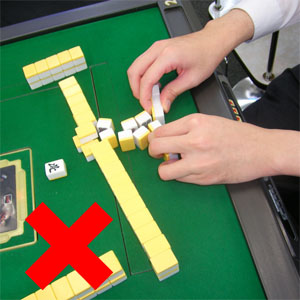
\includegraphics[width=8cm]{etiquette-6.png}
	\caption{Типичная ошибка при открытии руки}
\end{figure}

Даже если стол решит не штрафовать игрока и просто перенабрать тайлы --- это приведет к потере времени. Кроме того, открывая тайлы сразу игрок может быстрее понять потенциалы своей руки, что сэкономит время на обдумывание первого хода, а если при этом тайлы еще и сортировать пока другие игроки берут свои, то время экономится еще и на сортировке.

\begin{figure}[H]
	\centering
	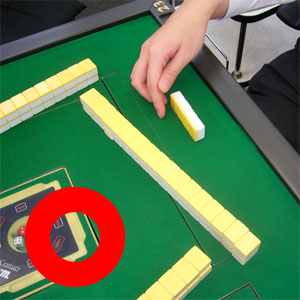
\includegraphics[width=8cm]{etiquette-7.png}
	\caption{Правильный набор руки}
\end{figure}

Отдельно стоит упомянуть что игроки должны не забывать взять 13 тайл, а дилер не должен делать первый ход пока все игроки не взяли тайлы. Таким образом, именно дилер должен убедиться что у всех игроков 13 тайлов в начале раздачи и указать на это игрокам, которые забыли взять последний тайл (чаще всего забывает взять игрок на севере). Нет необходимости пересчитывать тайлы в руках игроков --- достаточно взглянуть на живую стену, в ней должен быть только один свободный тайл в нижнем ряду. 

\subsection{Процесс игры}

\subsubsection{Взятие тайлов из стены}

Рекомендуется следить за тем, чтобы не показывать свои тайлы другим игрокам. Общая рекомендация --- не делать лишних движений. Например, не следует поворачивать тайл, пока он не окажется в зоне руки.

\begin{figure}[H]
	\centering
	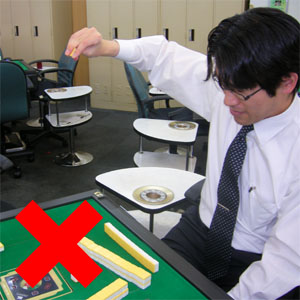
\includegraphics[width=8cm]{etiquette-8.png}
	\caption{Не делайте так при взятии}
\end{figure}

Не встраивайте взятый тайл в руку сразу же --- в случае победы вам не будет засчитано пинфу или фу. Взятый тайл следует располагать справа от руки (с небольшим зазором) для правшей, слева --- для левшей. Допустимо расположить взятый тайл сверху игровой руки, поставив его на бок, однако следует избегать этого при игре наборами для автостола, поскольку магнит внутри тайла может развернуть тайл лицевой стороной к игрокам. Встраивать тайл в руку можно после сброса.

\subsubsection{Сброс тайлов}

Старайтесь выполнять сброс тайла так, чтобы все игроки видели значение тайла одновременно. Некоторые игроки при сбросе тайла перекрывают видимость игроку слева, это приводит к тому, что игрок справа (чей ход следующий) видит тайл раньше игрока слева и делает свое взятие, а игрок слева, увидев тайл позже, решает объявить на нем пон. Задержка приведет к тому, что игрок либо не объявит пон, подумав что следующий тайл уже взяли (хотя технически он имеет на это право), либо к тому что пон будет объявлен но игрок справа будет знать какой тайл в стене. Лучше такого избегать, в том числе, игрокам не стоит торопиться брать свой тайл после сброса слишком быстро, стоит убедиться что все игроки за столом точно видели сброс и не делают на нем объявления. 

Сброс следует делать по шесть тайлов в ряд (следить за тем чтобы начинать второй ряд не раньше --- после пятого тайла, и не позже --- после седьмого):

\begin{figure}[H]
	\centering
	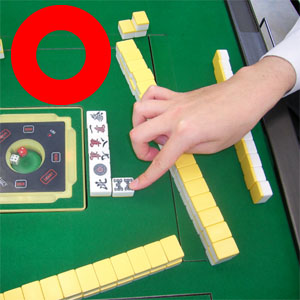
\includegraphics[width=8cm]{etiquette-9.png}
	\caption{Расположение дискарда}
\end{figure}

В случае если в третьем ряду уже лежит 6 тайлов, а тайлы в стене еще остались, следует продолжить третий ряд, а не начинать четвертый.

\subsection{Объявления}

\subsubsection{Объявления понов и чи}

При объявлении пона с игроков справа или напротив игроку следует стараться сделать объявление как можно быстрее, чтобы игрок, чей ход в данный момент, не успел взять и посмотреть тайл или не объявил чи. Если очевидно, что игрок не торопится сделать взятие и раздумывает над чи --- также следует объявить пон как можно раньше, чтобы игрок не засветил тайлы в своем сете. Если игрок успел сказать «чи», допустимо сказать «пон», но следует сделать это до того как игрок открыл два своих тайла. Недопустимо объявлять пон исходя из того, что кто-то решил взять чи: игроку, который хочет объявить чи, следует выждать пару секунд, убедившись что никто не планирует объявлять пон, и только потом делать объявление.

После объявления (которое нужно сделать достаточно громко, убедившись что все услышали и никто не пытается взять свой тайл и продолжить игру) следует последовательно открыть два тайла из руки, потом отложить их справа от руки, далее забрать объявленный тайл, потом сформировать сет, корректно повернув взятый тайл, чтобы он указывал на игрока, с которого он был взят, отложить сет в правый угол стола, и наконец произвести снос.

\begin{figure}[H]
	\centering
	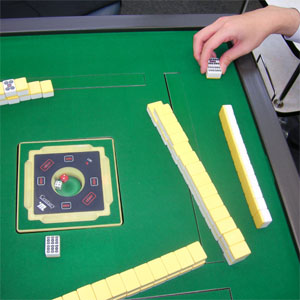
\includegraphics[width=8cm]{etiquette-10.png}
	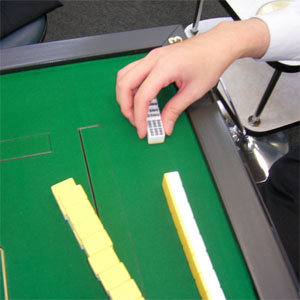
\includegraphics[width=8cm]{etiquette-11.png}
	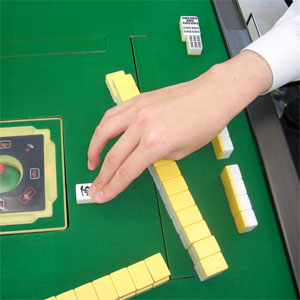
\includegraphics[width=8cm]{etiquette-12.png}
	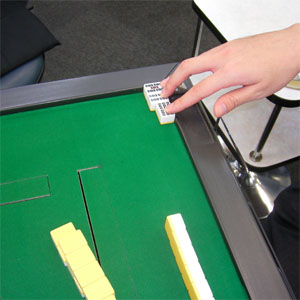
\includegraphics[width=8cm]{etiquette-13.png}
	\caption{Правильная последовательность объявление сета}
\end{figure}

Некоторые игроки открыв два тайла делают снос, а затем завершают формирование сета. Следует отказаться от этой практики по двум причинам:
\begin{itemize}
	\item На нашем сносе тоже может быть объявление и одновременно несколько тайлов будут забираться из сносов, может произойти путаница;
	\item Можно банально забыть забрать тайл из сноса и получить мертвую руку.
\end{itemize}

Такой порядок может наказываться вежливым указанием (в случае повторения --- штрафом)

Некоторые игроки открывают сразу три тайла --- объявляемые и тот, который пойдет в снос. Следует отказаться от этой практики, поскольку иногда по такому открытию неочевидно, какие именно тайлы мы объявляем, а какой готовимся снести (например если на сносе 2 открыть 134). Если игрок еще не решил, что именно будет сносить, следует сначала подумать, и открывать сет только после того как решение принято. Открытие трех тайлов сразу может наказываться вежливым указанием и штрафом в случае повторения.

В случае если игрок случайно открыл тайлы, которые не завершают сет, и это было быстро замечено им или указано на это другими игроками, необходимо либо открыть корректные тайлы, либо, если их в руке нет, отменить объявление. Такое поведение наказывается вежливым укаанием так не делать, но может и повлечь за собой штраф в случае повторения ситуации.

В случае если никто не заметил некорректного объявления сразу, игра была продолжена, а ошибка была замечена впоследствии --- игроку назначают мертвую руку.

При объявлении нескольких сетов можно выкладывать их в правом углу как справа налево, так и снизу вверх, но рекомендуется выкладывать именно снизу вверх, т.к. при трех и более объявлениях когда тайлы выложены справа налево мы будем перекрывать их видимость для других игроков при своем взятии из стены, а объявления должны быть всегда и всем видны. Не следует смешивать порядок --- класть второе объявление сверху над первым, а третье слева от него, не следует класть более ранние объявления левее/выше более поздних, всегда должно быть однозначно видно, в каком порядке были сделаны объявления в раздаче.

На последнем сбросе в раздаче никакие объявления кроме объявления победы недопустимы.

\subsubsection{Объявление канов}

Открытие канов относительно похоже на объявление понов --- последовательность действий при объявлении следует соблюдать аналогичным образом. Рассмотрим отличия, характерые именно для канов.

Закрытый кан или апгрейд пона до кана возможны только после взятия из стены (живой или мертвой), нельзя объявить никакой кан сразу после объявления пона/чи.

% TODO уточнить по итогу обсуждений

Если по правилам индикаторы открываются сразу --- то после того как игрок объявил кан и показал корректно все 4 тайла (при закрытом кане), 3 тайла при открытом кане, 1 тайл при апгрейде пона до кана (если не был объявлен рон чанкан) игрок в чьей стене находится новый индикатор сразу переворачивает новый. Игрок объявивший кан сформировав его в правом углу обязательно берет тайл замены прежде чем сделать снос, если игроки видят что он готовиться снести тайл они должны напомнить ему о необходимости взять тайл замены. Открытые индикаторы будут применятся в том числе при победе на тайле замены. В случае игры по олдовым правилам (сейчас такие приняты в онлайне), при открытых канах индикаторы открываются только после сноса игрока или объявления им следующего кана. Если на сносе будет объявлена победа --- индикатор будет действовать для выигравшего, если будет победа по риншану --- то индикатор последнего кана не действует для победившего по риншану (если последний кан не закрытый, впрочем вообще вопрос дискуссионный, но здесь описано как в онлайне), в случае если после открытого кана был объявлен апгрейд пона до кана с последующим роном чанканом --- для победившего будет открыт индикатор от первого кана, но не от второго. В связи с тем что, как видите, есть много нюансов с порядком открытия индикаторов --- предлагается за базовые правила брать рулсет ема где открытие индикаторов происходит сразу же (кроме чанкана), что значительно упрощает понимание порядка действий и исключает возможные двусмысленные трактовки разными игроками.

Нужно не забывать, что после того, как игрок объявил тайл и взял тайл замены, живая стена стала на один тайл короче, т.к. в мертвой стене всегда 14 тайлов. Не рекомендуется делать каких-либо манипуляций, чтобы обозначить это, особенно если до конца раздачи еще далеко --- как правило это лишняя трата времени. Кроме того, можно запутаться и переместить в мертвую стену не тот тайл. В идеале, когда раздача будет близиться к концу, игрокам нужно прикинуть, какой тайл на данный момент будет последним, после чего можно слегка его подвинуть и указать всем условно что «последний тайл в раздаче вот этот». Если кто-то из игроков настаивает на снятии этого тайла для более простого восприятия --- игрок в чьей стене на данный момент находится последний тайл аккуратно его перемещает в конец живой стены, и все следят, чтобы ничего не было перепутано.

Также кратко стоит упомянуть важный момент --- кан можно объявить только если в живой стене есть хотя бы один тайл --- т.к. этот тайл нужно переместить в мертвую стену (а если тайлов в живой стене нет --- то перемещать нечего). При этом последнее взятие в игре будет из мертвой стены, в случае победы на нем будет засчитан риншан, но не хайтей (риншан и хайтей не сочетаются). При объявлении закрытого кана пятерок при игре с акадорами --- красная пятерка должна быть среди видимых, чтобы при подсчете стоимости руки ее не забыли посчитать.

\subsubsection{Объявление риичи}

Крайне важно соблюдать корректный порядок объявления: 
\begin{itemize}
	\item Громко (чтобы все услышали и обратили внимание) сказать «риичи»;
	\item Снести тайл боком в дискард
	\item Убедиться, что на сброшенном тайле не объявлена победа
	\item Положить ставку риичи перед дискардом.
\end{itemize}

\begin{figure}[H]
	\centering
	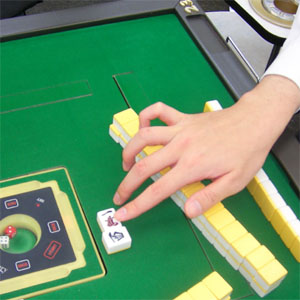
\includegraphics[width=8cm]{etiquette-14.png}
	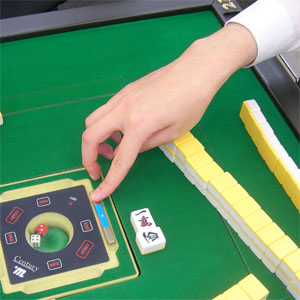
\includegraphics[width=8cm]{etiquette-15.png}
	\caption{Объявление риичи}
\end{figure}

Если тайл был взят в любой сет --- нужно не забыть повернуть свой следующий сброс (если забыли --- сразу, как только ошибка была обнаружена, всем столом восстановить последовательность и повернуть правильный тайл). Некорректный порядок объявления риичи приводит к тому, что объявление не засчитывается. Не допускается объявлять риичи после сброса (ситуация «никому не нужно? тогда риичи»), такое риичи также не засчитывается, а за пустое объявление можно получить вежливое указание так не делать, а при повторении --- штраф. 

Игрок справа перед своим следующим взятием должен дождаться, пока мы выполним все действия (повернем тайл, положим палочку), и только после этого делать взятие, то же касается игроков, которые хотят на нашем тайле сделать объявление --- можно сказать пон/кан, но обязательно прежде чем забирать тайл дождаться, пока игрок с риичи положит палочку. При объявлении победы ждать не требуется, т.к. палочку риичнувший игрок в этом случае не кладет, победу нужно объявлять сразу.

После объявления риичи игроку крайне нежелательно касаться взятым из стены тайлом своей руки, чтобы избежать подозрений в изменении руки. Взятые тайлы можно смотреть не ставя тайл в руку, также допустимо ставить рядом с рукой (справа для правшей, слева для левшей), но не касаясь ее или располагать тайл сверху руки боком (в случае игры на трансляции так делать даже рекомендуется). Не стоит класть невыигрышные тайлы в открытую рядом с рукой. Если тайл невыигрышный, открывать его нужно именно в сносе, чтобы игроки не подумали, что вы объявляете победу --- за подобное расположение тайла полагается вежливое указание так не делать, а в случае повторения может быть назначен штраф.

\begin{figure}[H]
	\centering
	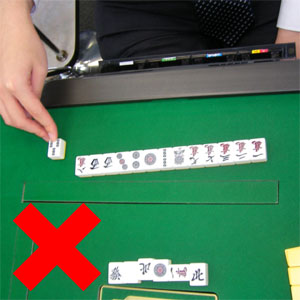
\includegraphics[width=8cm]{etiquette-16.png}
	\caption{Объявление победы при риичи}
\end{figure}

Игрок с риичи может объявить валидный кан, в этом случае он сначала говорит кан, потом кладет взятый тайл в открытую рядом с рукой и дополняет его тремя тайлами из руки, чтобы сформировать закрытый кан.

Игроки с риичи при ничьей обязательно показывают состояние своей руки, чтобы все могли убедиться, что у них есть темпай, даже если после риичи игроку по каким-то причинам была объявлена мертвая рука (например при некорректном объявлении победы). Игрок с мертвой рукой будет считаться нотен, показ руки необходим, чтобы убедиться, что риичи было корректное (в руке был темпай), а также что после риичи не было некорректных объявлений канов. В случае если что-либо из этого было нарушено, игрок получает чомбо.

Риичи можно объявить только если в живой стене осталось не меньше четырех тайлов (если при отсутствии каких либо объявлений у объявляющего риичи игрока будет хотя бы одно взятие). 

\subsection{Победа и ничья}

\subsubsection{Объявление победы}

При объявлении победы следует соблюдать корректный порядок действий:

\begin{itemize}
	\item Объявить «рон» достаточно громко чтобы все услышали и убедиться что никто не пытается продолжить игру, взяв тайл из стены или объявив пон на том же тайле;
	\item Осторожно открыть всю руку;
	\item В случае победы с риичи --- открыть и показать всем урадоры;
	\item Перечислить все комбинации в руке, назвать количество дор и итоговое количество хан и фу.
\end{itemize}

Не разрешается забирать выигрышный тайл из сброса другого игрока. При нарушении может быть назначение вежливое указание (при повторном нарушении --- штраф). Обоснование заключается в том, что набросивший игрок может оспорить необходимость платить вам, т.к. в его сбросе нет вашего выигрышного тайла. Кроме того, возможны случаи когда тайл наброшен в две и более рук. Если наброс произведен дорой следует не забыть посчитать ее при перечислении количества дор в руке.

\begin{figure}[H]
	\centering
	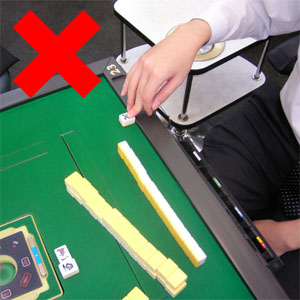
\includegraphics[width=8cm]{etiquette-17.png}
	\caption{Объявление рона}
\end{figure}

В случае выигрыша со стены также придерживаемся строгой последовательности:

\begin{itemize}
	\item Объявить «цумо» достаточно громко чтобы все услышали и убедиться что никто не пытается продолжить игру;
	\item Осторожно открыть всю руку;
	\item В случае победы с риичи --- открыть и показать всем урадоры;
	\item Перечислить все комбинации в руке, назвать количество дор и итоговое количество хан и фу.
\end{itemize}

Победный тайл не следует встраивать в руку, нужно положить его рядом с рукой справа (с небольшим зазором) для правшей, слева --- для левшей. 

\begin{figure}[H]
	\centering
	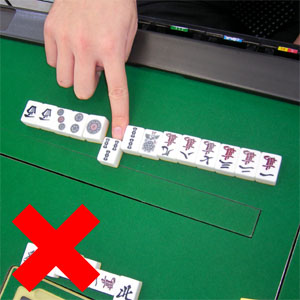
\includegraphics[width=8cm]{etiquette-18.png}
	\caption{Объявление цумо}
\end{figure}

Рука должна быть отсортирована:

\begin{figure}[H]
	\centering
	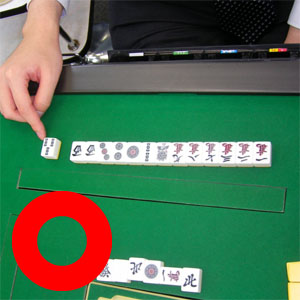
\includegraphics[width=8cm]{etiquette-19.png}
	\caption{Сортировка руки}
\end{figure}

Не следует класть победный тайл перед рукой, особенно если стена перед вами полностью разобрана --- другими игроками это может быть воспринято как снос, на нем могут попытаться объявить победу.

\begin{figure}[H]
	\centering
	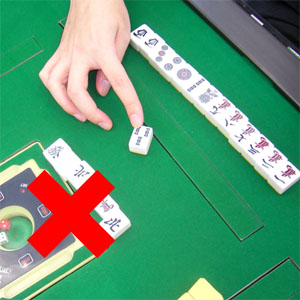
\includegraphics[width=8cm]{etiquette-20.png}
	\caption{Тайл перед рукой}
\end{figure}

В случае если игрок пытается объявить цумо положив тайл за область своей стены ему следует вынести вежливое указание так не делать, но руку засчитать. 

После объявления стоимости руки стоит не забыть упомянуть про хонбу, если она есть, и по возможности назвать итоговую стоимость с учетом хонбы («семь семьсот, с учетом двух хонб --- восемь триста» или «семьсот, тысяча триста, одна хонба, итого, восемьсот, тысяча четыреста»).

Объявление стоимости при цумо следует начинать с меньшего значения во избежание путаницы (сравните --- «2 хан, 30 фу, пятьсот, тысяча» и «2 хан, 30 фу, тысяча пятьсот»).

\subsubsection{Ничья}

При ничьей темпай-игроки показывают свои руки. Если игрок не объявлял риичи, он не обязан показывать руку, может объявить нотен и закрыть ее, даже если его рука открыта до одного тайла\footnote{Это может быть истиной, например при ожидании в тайл, пон которого уже открыт у игрока, но даже если это не так --- игрок в любом случае вправе закрыть руку, объявив нотен}. Объявление темпаев/нотенов следует производить поочередно, начиная с дилера (затем юг, запад, север). Открытие руки вне очереди не наказывается, но игрок имеет право не показывать состояние своей руки, пока игроки до него не покажут свое.

Дилеру может быть выгодно показать нотен если у определенных игроков тоже нотен (например, чтобы завершить игру), но другие игроки не обязаны раскрывать ему состояние руки, пока он не объявит свое.

\subsubsection{Расчеты за победу/ничью}

После того как победивший игрок назвал стоимость своей руки (см подробности в разделе 6), игроки, которые делают выплаты, должны положить соответствующую сумму на стол рядом с собой. Не следует класть палочки пближе к выигравшему --- в случае цумо когда так сделают несколько игроков будет непонятно кто сколько положил. При расчетах следует стремиться к тому, чтобы было использовано как можно меньше палочек --- при победе в 3900 следует дать пятитысячную палочку и попросить сдачу в тысячу сто. По возможности, размен стоит производить палочками, которые уже лежат на столе, например если игрок собрал по цумо 700/1300 дилер может дать две тысячных палочки и забрать в качестве сдачи 700 очков, которые дал другой игрок, но подобные действия при расчете следует озвучивать вслух. В случае, если на столе были риичи палочки --- победившему игроку (в случае дабл-рона --- имеющему на них право игроку), следует сразу подвинуть их к себе, чтобы они не смешивались с очками, которыми будут производиться выплаты. Также после выплат игрокам стоит убедиться, что у них есть хотя бы одна тысячная палочка для объявления риичи, и в случае ее отсутствия попросить у других игроков размен.

\begin{figure}[H]
	\centering
	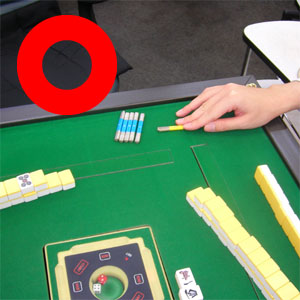
\includegraphics[width=8cm]{etiquette-21.png}
	\caption{Расчет палочками}
\end{figure}

В случае, если при объявлении риичи обнаружилось, что тысячной палочки нет --- также стоит попросить размен, желательно непосредственно перед объявлением риичи а не в момент когда кладется палочка, как на картинке выше.

Только после того как очки были проверены всеми игроками и учтены, допускается перевернуть тайлы и приступить к перемешиванию тайлов, любые изменения в расчетах после этого момента производиться не должны. Если все за столом согласны, например игроки вспомнили что забыли отметить чью-то риичи палочку, или недосчитали дору, допустим перерасчет, но только если все игроки за столом действительно помнят, что было именно так, и не против внести изменения.

\subsection{Поведение за столом}

Следует обратить внимание на то, как вы сидите: не скрещивайте руки, не кладите ногу на ногу, не ставьте локти на стол и не подпирайте голову рукой:

\begin{figure}[H]
	\centering
	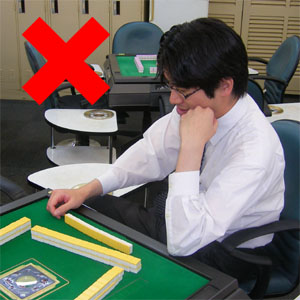
\includegraphics[width=8cm]{etiquette-22.png}
	\caption{Поза за столом}
\end{figure}

Держаться следует свободно, открыто, раскованно, нерабочую руку (для праворуких — левую и наоборот) следует класть на колено.

\begin{figure}[H]
	\centering
	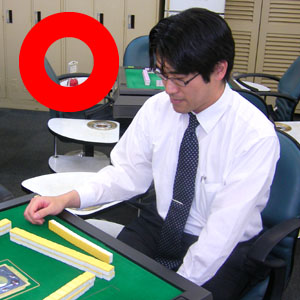
\includegraphics[width=8cm]{etiquette-23.png}
	\caption{Поза за столом}
\end{figure}

Не следует закрывать свою руку в процессе игры, в частности --- не следует закрывать руку после объявления риичи. Если рука была закрыта, другие игроки могут счесть вашу руку за часть стены и сделать взятие из нее --- в этом случае вы сами будете виноваты в том, что ваша рука признана мертвой.

\begin{figure}[H]
	\centering
	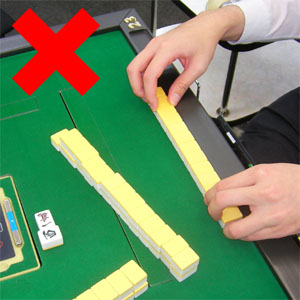
\includegraphics[width=8cm]{etiquette-24.png}
	\caption{Рука при риичи}
\end{figure}

Повторим также еще раз --- необходимо делать все объявления громко и четко, несоблюдение этого правила может быть наказано вежливым указанием или штрафом в случае повторения.
